%	This is written by Zhiyang Ong as a template for writing reports.

%	The MIT License (MIT)

%	Copyright (c) <2014> <Zhiyang Ong>

%	Permission is hereby granted, free of charge, to any person obtaining a copy of this software and associated documentation files (the "Software"), to deal in the Software without restriction, including without limitation the rights to use, copy, modify, merge, publish, distribute, sublicense, and/or sell copies of the Software, and to permit persons to whom the Software is furnished to do so, subject to the following conditions:

%	The above copyright notice and this permission notice shall be included in all copies or substantial portions of the Software.

%	THE SOFTWARE IS PROVIDED "AS IS", WITHOUT WARRANTY OF ANY KIND, EXPRESS OR IMPLIED, INCLUDING BUT NOT LIMITED TO THE WARRANTIES OF MERCHANTABILITY, FITNESS FOR A PARTICULAR PURPOSE AND NONINFRINGEMENT. IN NO EVENT SHALL THE AUTHORS OR COPYRIGHT HOLDERS BE LIABLE FOR ANY CLAIM, DAMAGES OR OTHER LIABILITY, WHETHER IN AN ACTION OF CONTRACT, TORT OR OTHERWISE, ARISING FROM, OUT OF OR IN CONNECTION WITH THE SOFTWARE OR THE USE OR OTHER DEALINGS IN THE SOFTWARE.

%	Email address: echo "cukj -wb- 23wU4X5M589 TROJANS cqkH wiuz2y 0f Mw Stanford" | awk '{ sub("23wU4X5M589","F.d_c_b. ") sub("Stanford","d0mA1n"); print $5, $2, $8; for (i=1; i<=1; i++) print "6\b"; print $9, $7, $6 }' | sed y/kqcbuHwM62z/gnotrzadqmC/ | tr 'q' ' ' | tr -d [:cntrl:] | tr -d 'ir' | tr y "\n"

%%%%%%%%%%%%%%%%%%%%%%%%%%%%%%%%%%%%%%%%%%%%%%


%%%%%%%%%%%%%%%%%%%%%%%%%%%%%%%%%%%%%%%%%%%
\section{Pipelined Processor Design}
\label{sec:PipelinedProcessorDesign}

%    Hennessy2012
%    Appendix C (pipelining)

%    Hennessy2007
%    Appendix A (pipelining)

%    Hennessy2003
%    Appendix A (pipelining)

%	6.27, microarch; 6.32; 6.36; 6.41; 6.42
%	3e, figure 6.17, microarchitecture, datapath



\begin{figure}[h]
\centering 
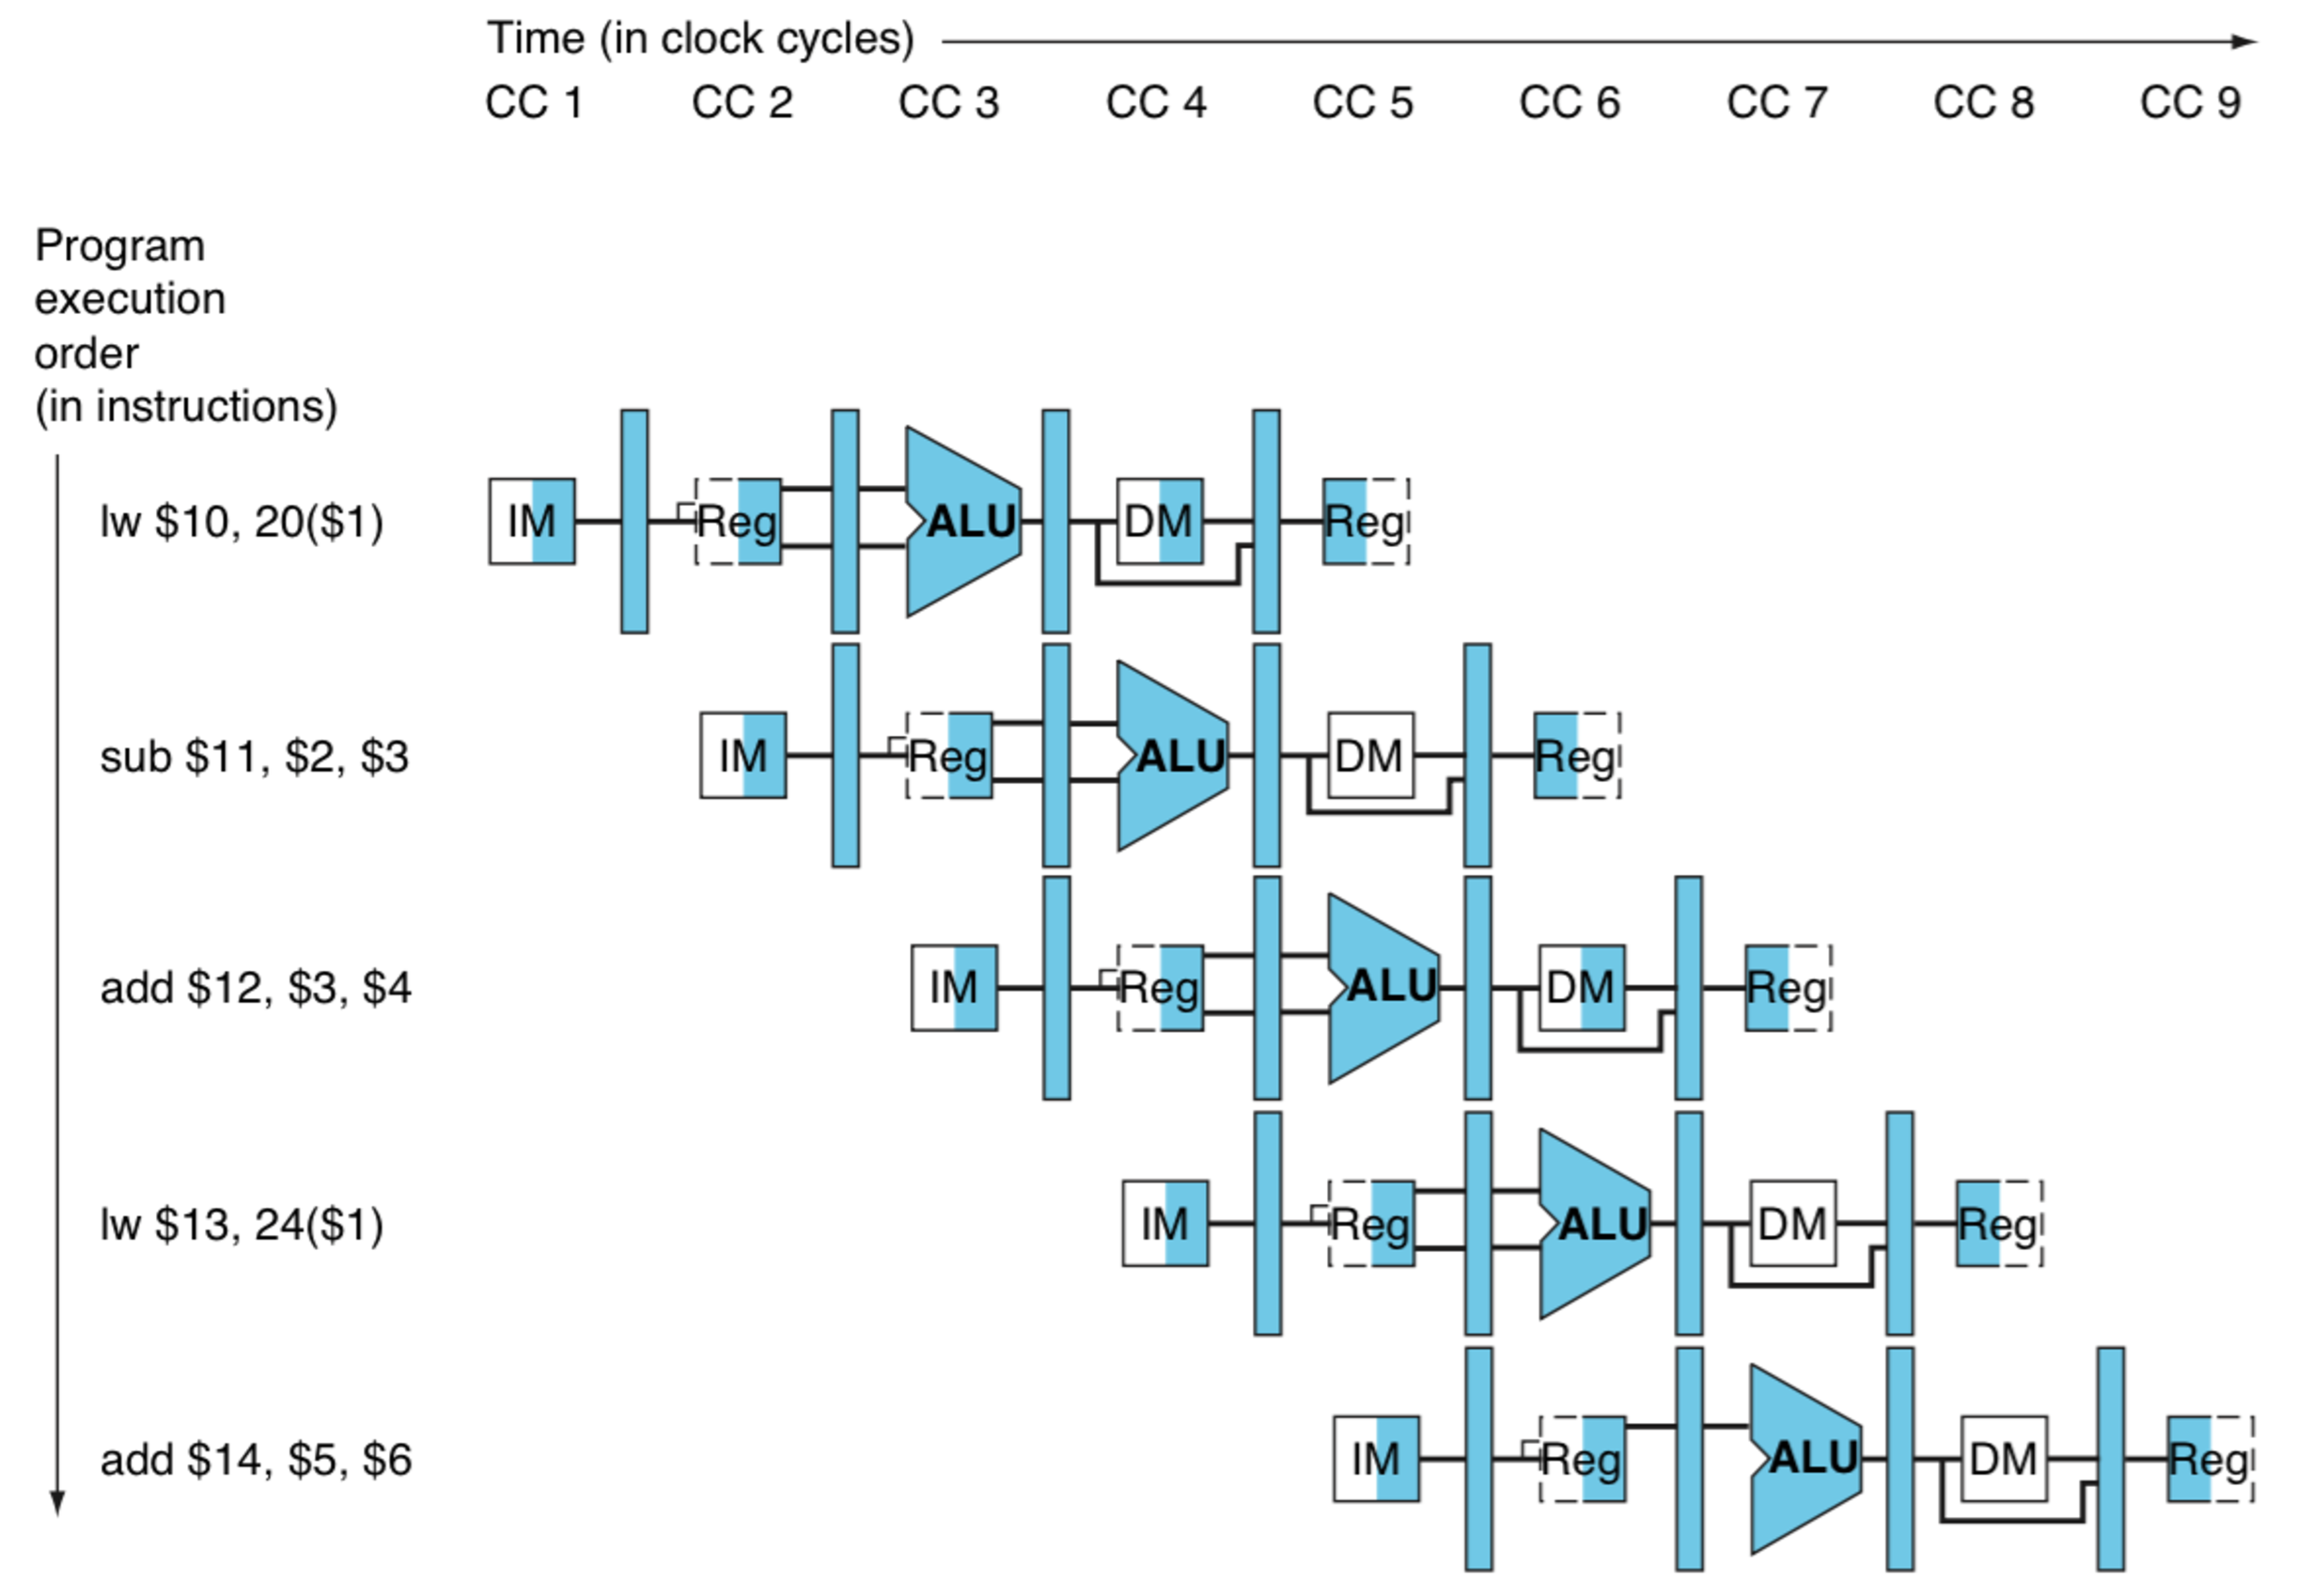
\includegraphics[width=6in]{./pics/pipelined-processor-pipelining}
\caption{A diagram of the datapath pipeline of the pipelined {\it MIPS} processor that shows the order of instruction execution for a sequence of five {\it MIPS} instructions. This datapath pipeline shows that each instruction would take at at least 5 clock cycles to execute \cite{Patterson2012}.}
\label{fig:pipelinedprocessorpipelining}
\end{figure}
%    pipeline diagram, 
%    Figure 6.19, Patterson2005, pp. 397
%    Figure 4.43, Patterson2012, pp. 357

Pipelining is a microarchitecture design technique that overlaps instructions, so that more hardware resources (or datapath components) in the datapath pipeline can be utilized. This allows computer programs to execute faster, and improve the performance of the pipelined processor. Figure \ref{fig:pipelinedprocessorpipelining} shows how the datapath of a pipelined {\it MIPS} processor can be pipelined to utilize more datapath components in each clock cycle. This pipelined {\it MIPS} processor fetches a new instruction every clock cycle, and each pipelined stage of the processor is processed in a clock cycle. At the next clock cycle, a given stage in the pipelined datapath would process the next instruction. An example of maximizing the usage of datapath components is shown in the fifth clock cycle, when all pipeline stages of the processor are being utilized. Therefore, pipelined processors are faster than multi-cycle processors, since the throughput of executing instructions is increased \cite{Patterson2012} to reduced the average execution time per instruction \cite{Hennessy2012}. \\

The performance speedup for a pipelined {\it MIPS} processor over an unpipelined {\it MIPS} processor is given as follows \cite{Hennessy2012}:\begin{equation}
\label{eqn:pipelinedprocessorspeedup}
{\rm performance\ speedup\ from\ pipelining} = \frac{\rm average\ execution\ time\ per\ unpipelined\ instruction}{\rm average\ execution\ time\ per\ pipelined\ instruction}
\end{equation}


\begin{figure}[h]
\centering 
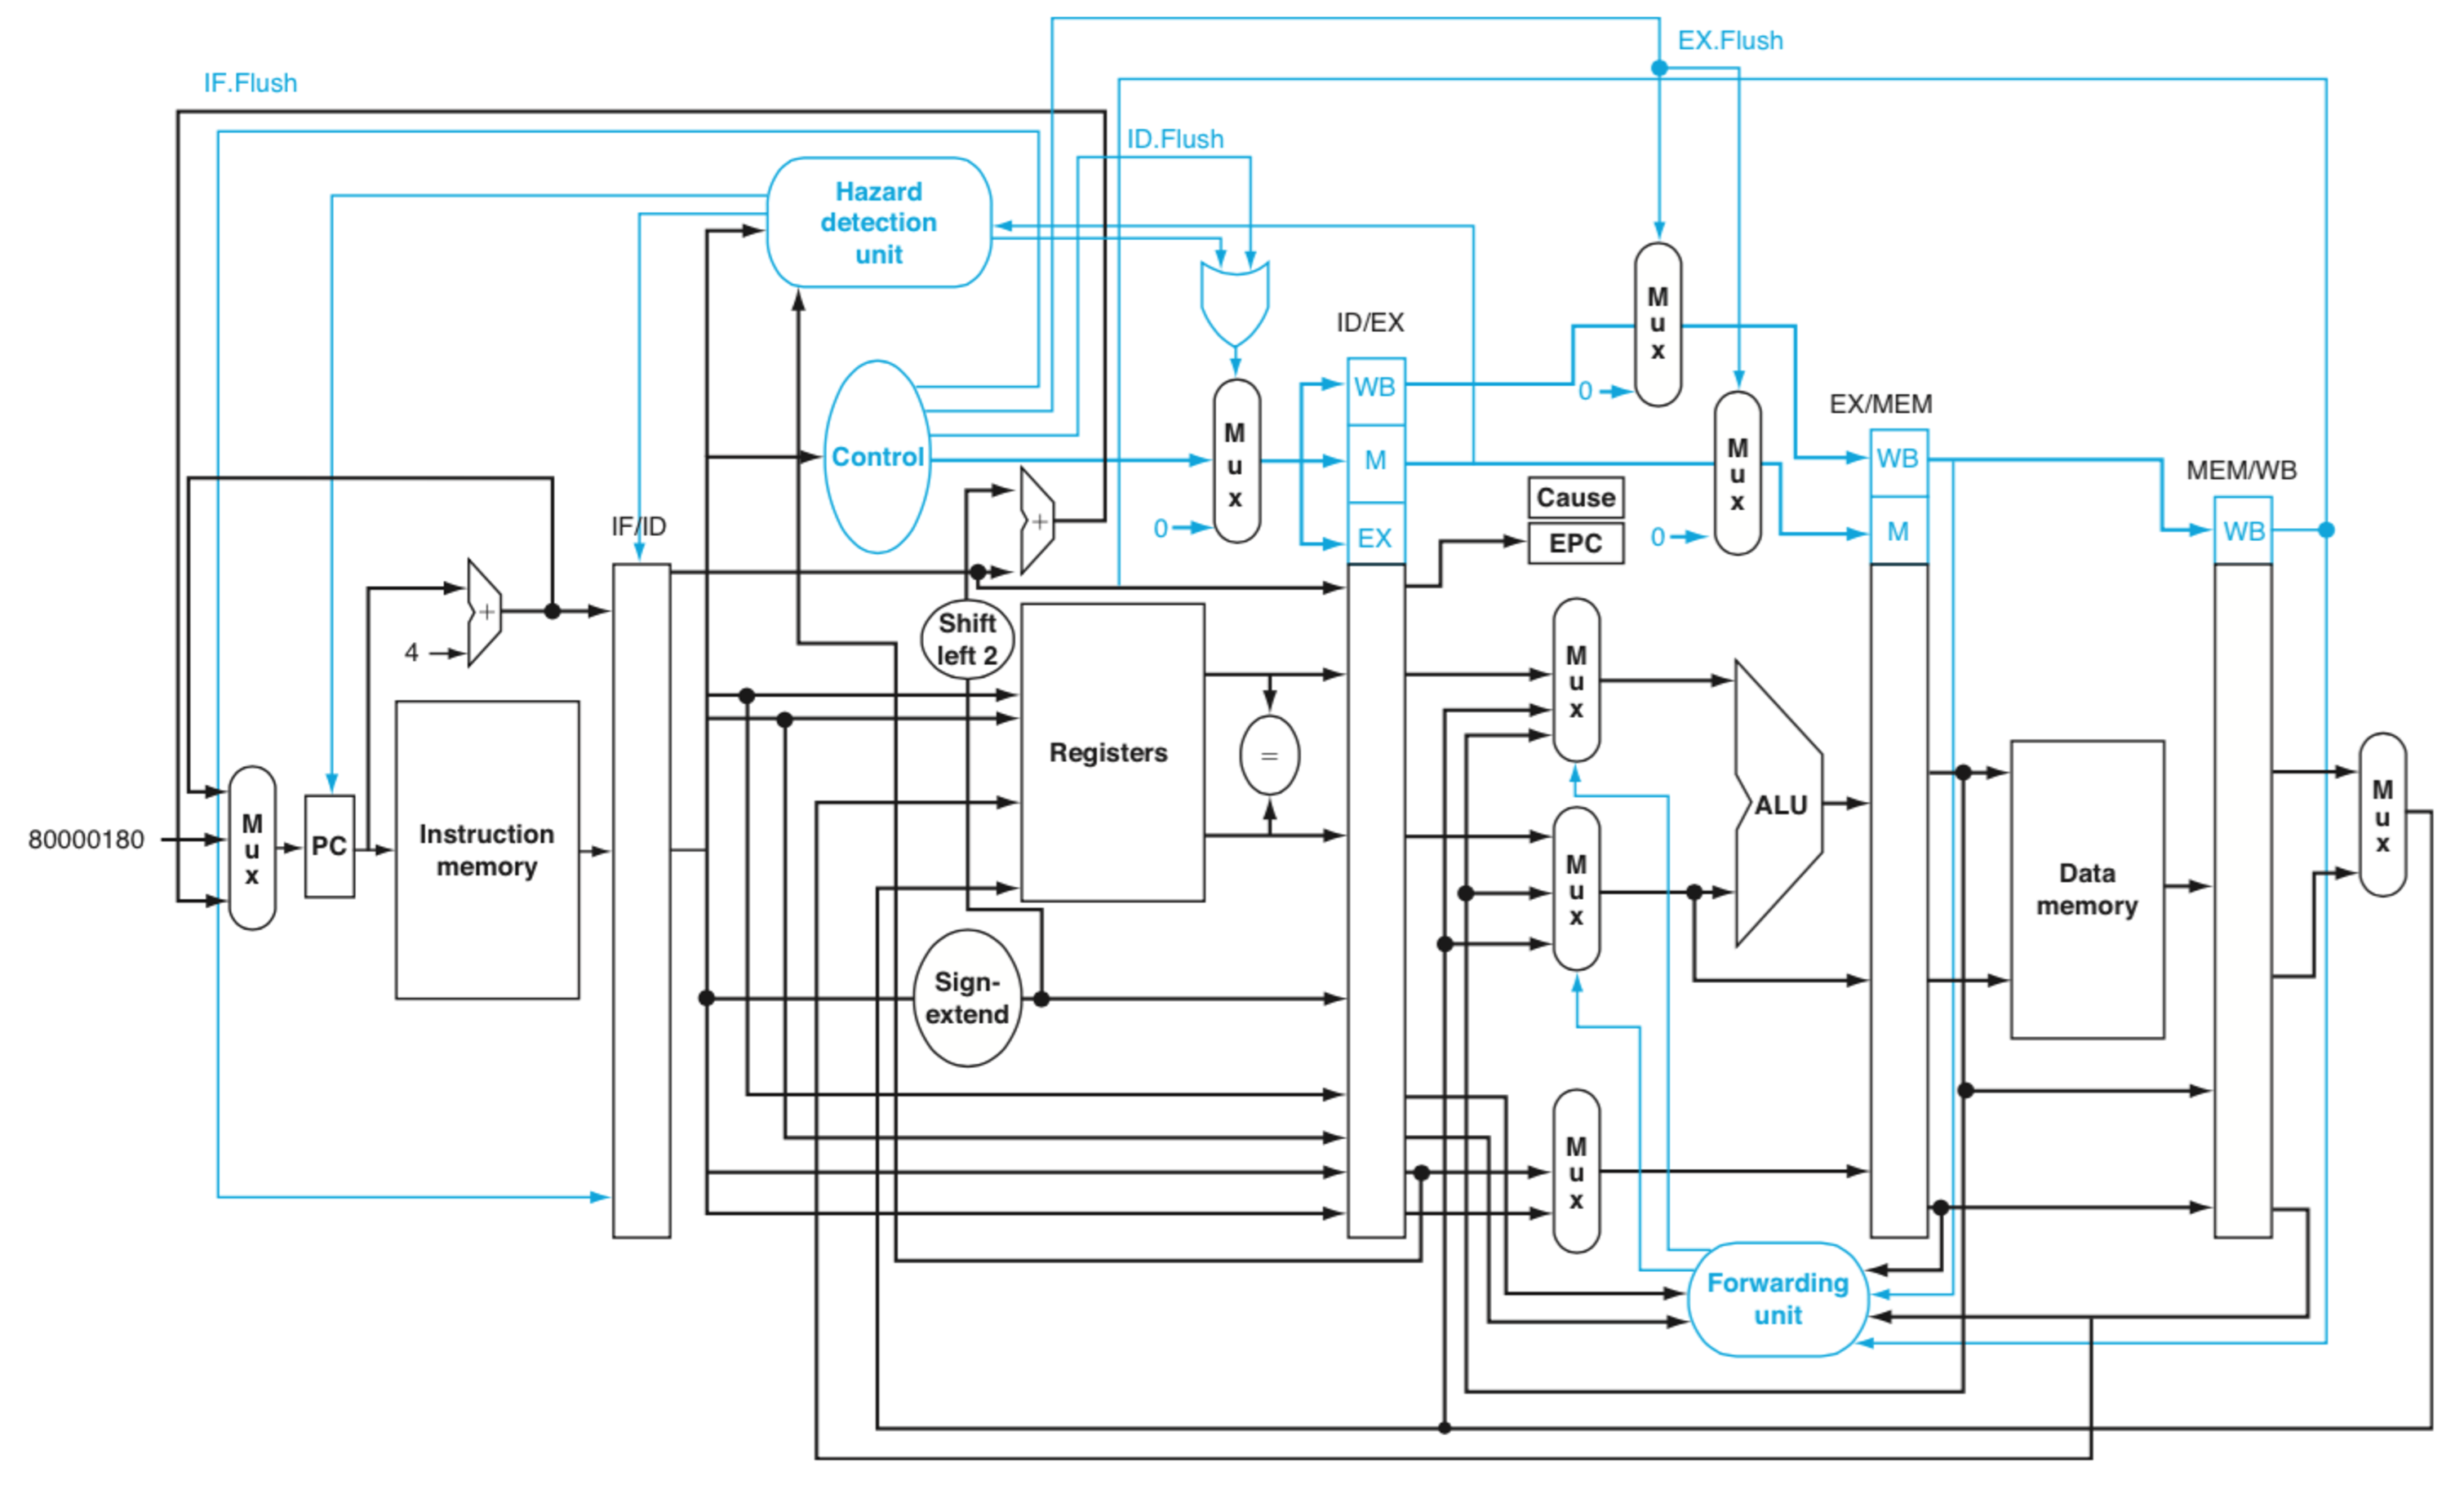
\includegraphics[width=6in]{./pics/pipelined-processor}
\caption{Microarchitecture of a pipelined {\it MIPS} processor that includes the datapath and the control path. It supports detection and handling of exceptions \cite{Patterson2012}.}
\label{fig:pipelinedprocessor}
\end{figure}
%    Datapath and control path 
%    Figure 6.42, Patterson2005, pp. 428
%    Figure 4.66, Patterson2012, pp. 387

%Figure \ref{fig:pipelinedprocessor} shows the microarchitecture of a pipelined {\it MIPS} processor that supports detection and handling of exceptions \cite{Patterson2012}. The pipelined stages of the pipelined {\it MIPS} processor's datapath are the same stages of the multi-cycle {\it MIPS} processor; see Section \ref{sec:MultiCycleProcessorDesign}. That is, the pipelined stages of the pipelined {\it MIPS} processor are: IF, ID, EX, MEM, and WB. In order to execute each pipelined stage in a clock cycle, pipelined registers are placed between pipelined stages to ensure that each pipelined stage will execute in one clock cycle.
Figure \ref{fig:pipelinedprocessor} shows the microarchitecture of a pipelined {\it MIPS} processor that supports detection and handling of exceptions \cite{Patterson2012}. The pipelined stages of the pipelined {\it MIPS} processor's datapath are the same stages of the multi-cycle {\it MIPS} processor; see Section \ref{sec:MultiCycleProcessorDesign}. That is, the pipelined stages of the pipelined {\it MIPS} processor are: IF, ID, EX, MEM, and WB. In order to execute each pipelined stage in a clock cycle, pipelined registers are placed between pipelined stages. \\

Pipeline hazards prevent the next instruction in the instruction sequence to execute during the clock cycle that it is supposed to. These pipeline hazards prevent the computer from achieving the ideal performance speedup. These hazards are categorized as follows \cite{Hennessy2012}: \vspace{-0.3cm}
\begin{enumerate} \itemsep -4pt
\item Structural hazards occur when multiple instructions need to use a datapath component in the same clock cycle. They prevent instructions from being overlapped in sequences, such that multiple instructions need to use a datapath component in the same clock cycle.
\item Data hazards occur when the computational results of an instruction are used or overwritten in subsequent instructions.
\item Control hazards occur when pipelined {\tt branch} and {\tt jump} instructions change the PC value.
\end{enumerate}


\begin{figure}[h]
\centering 
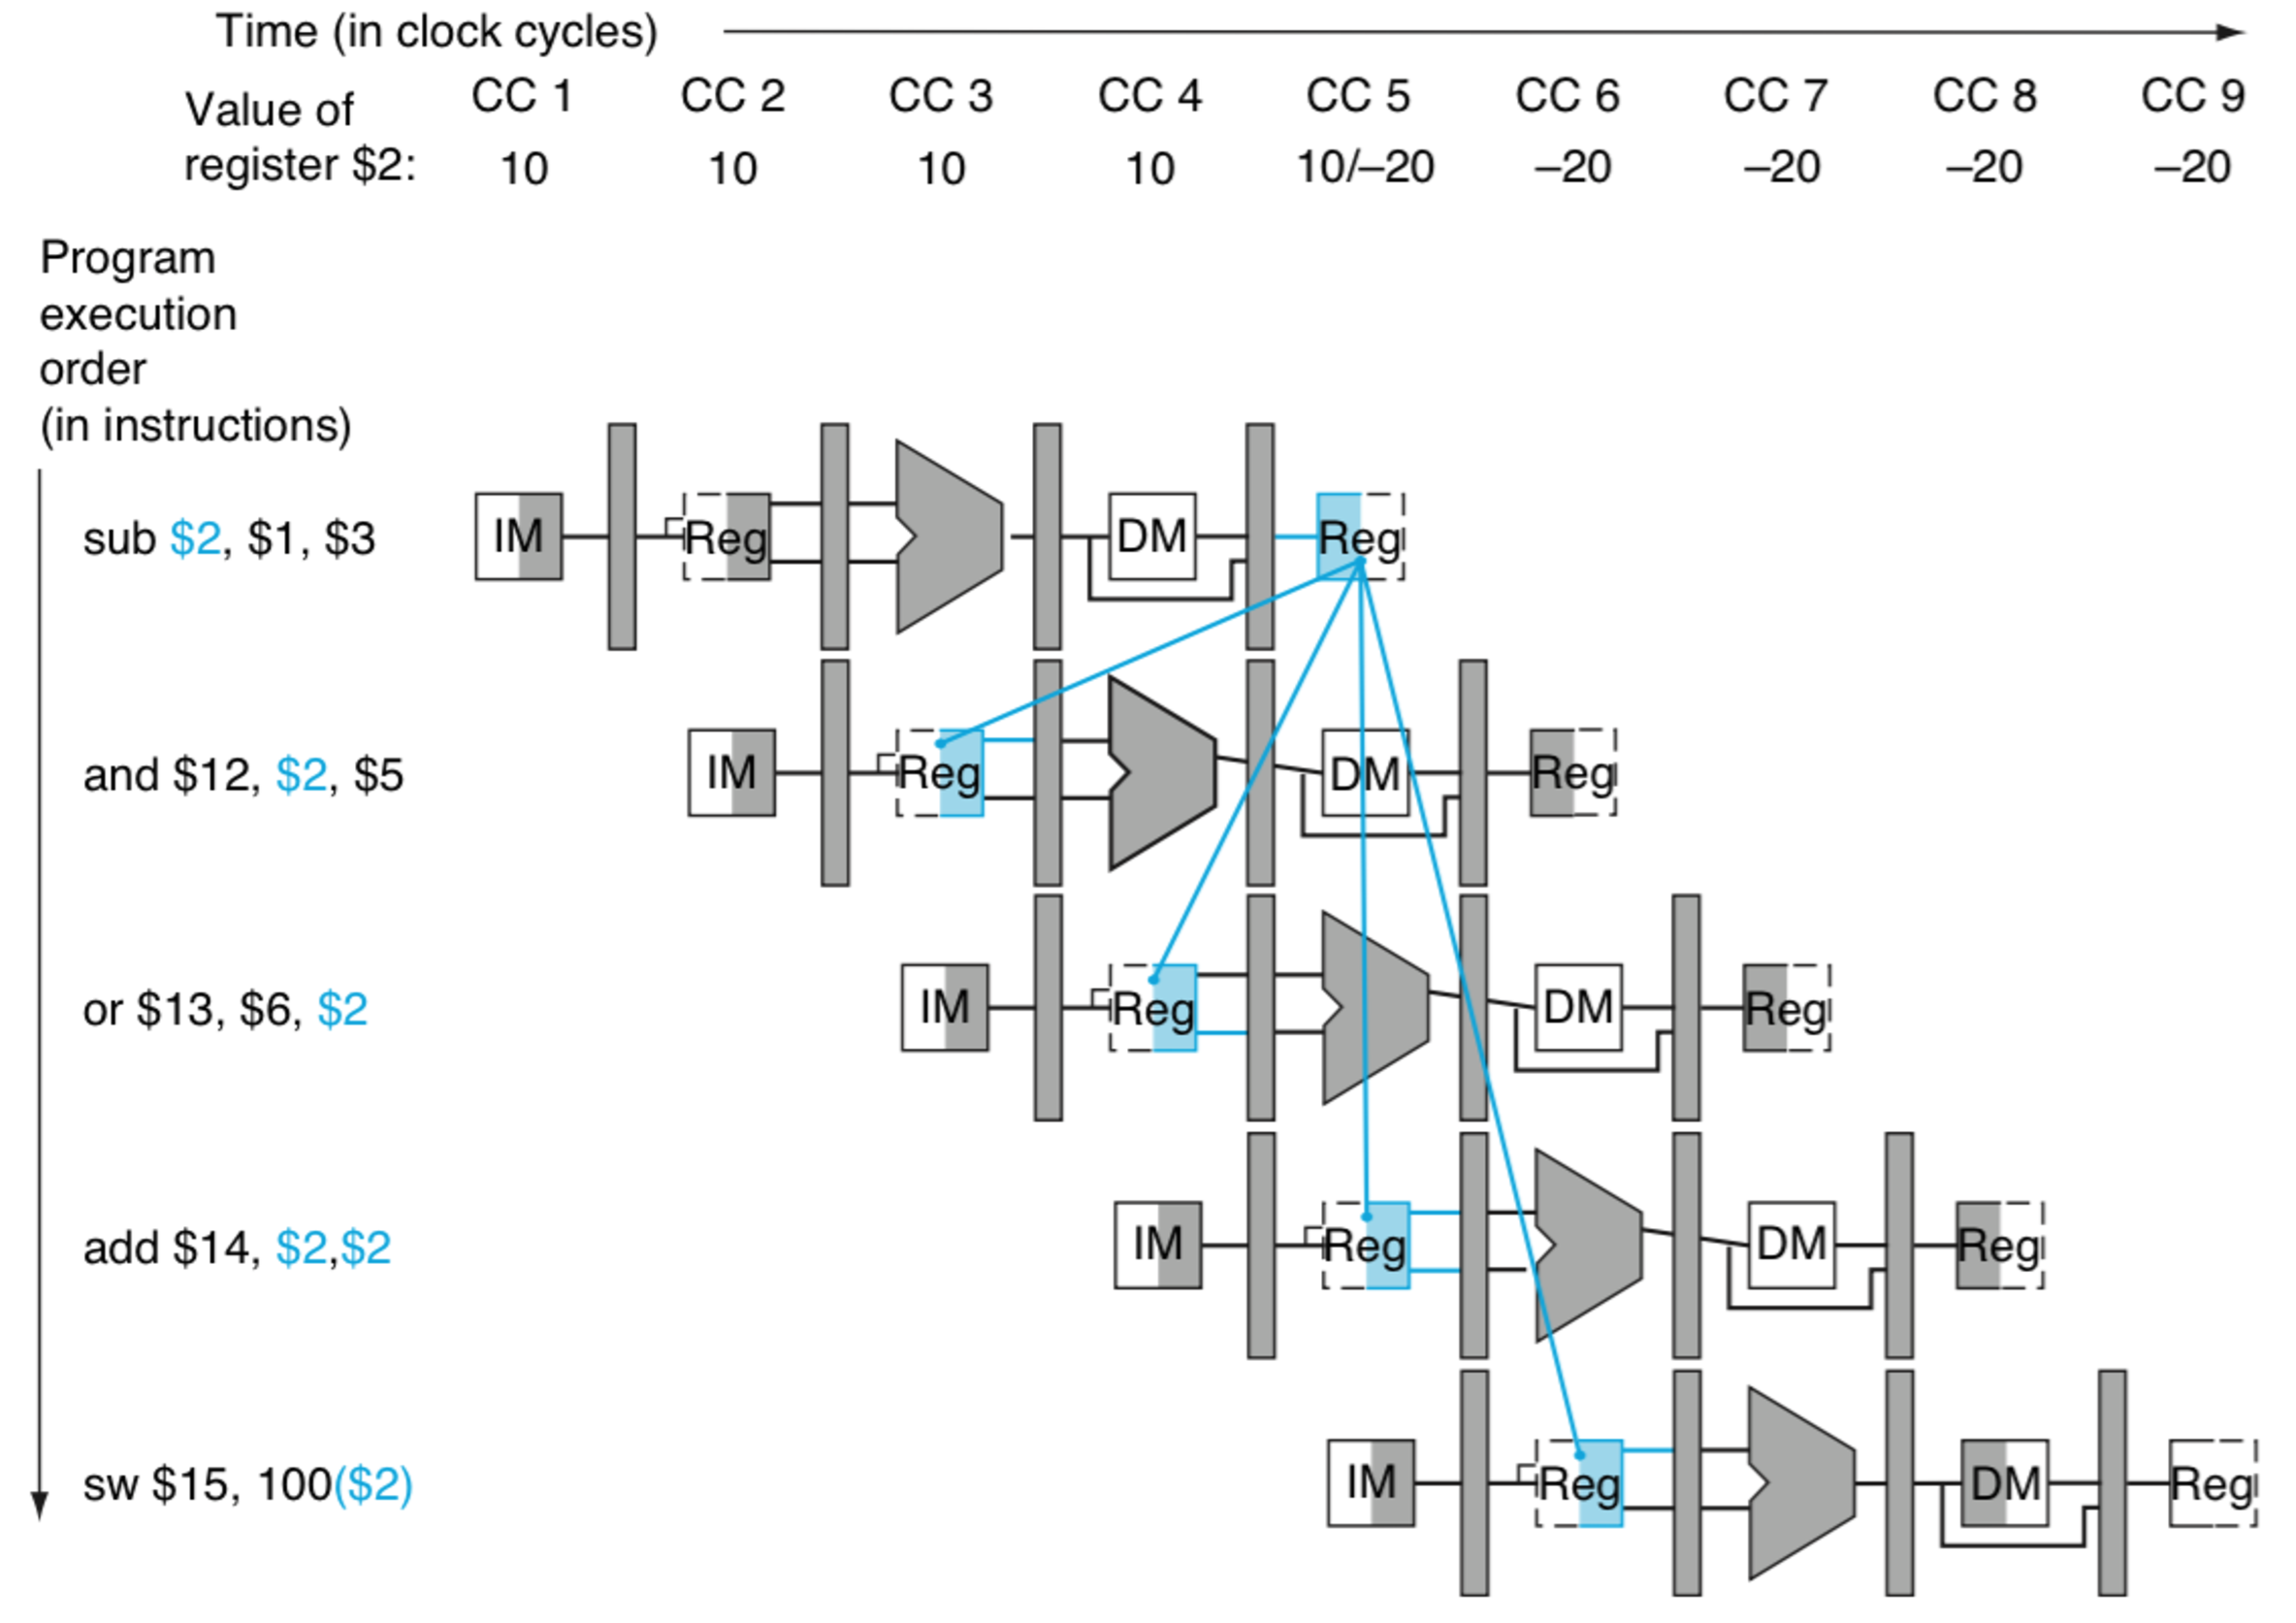
\includegraphics[width=6in]{./pics/pipelined-processor-raw-data-dependencies}
\caption{An example of Read-After-Write (RAW) data dependencies \cite{Hennessy2012,Shen2005a} between instructions in a snippet of a computer program \cite{Patterson2012}. There exists RAW data dependencies regarding register {\tt \$2} between the instruction {\tt sub \$2, \$1, \$3} and the following instructions: {\tt and \$12, \$2, \$5}; {\tt or \$13, \$6, \$2}; {\tt add \$14, \$2, \$2}; and {\tt sw \$15, 100(\$2)}. }
\label{fig:pipelinedprocessorrawdatadependencies}
\end{figure}
%    pipelined dependencies
%    Figure 6.28, Patterson2005, pp. 405
%    Figure 4.52, Patterson2012, pp. 364


\begin{figure}[h]
\centering 
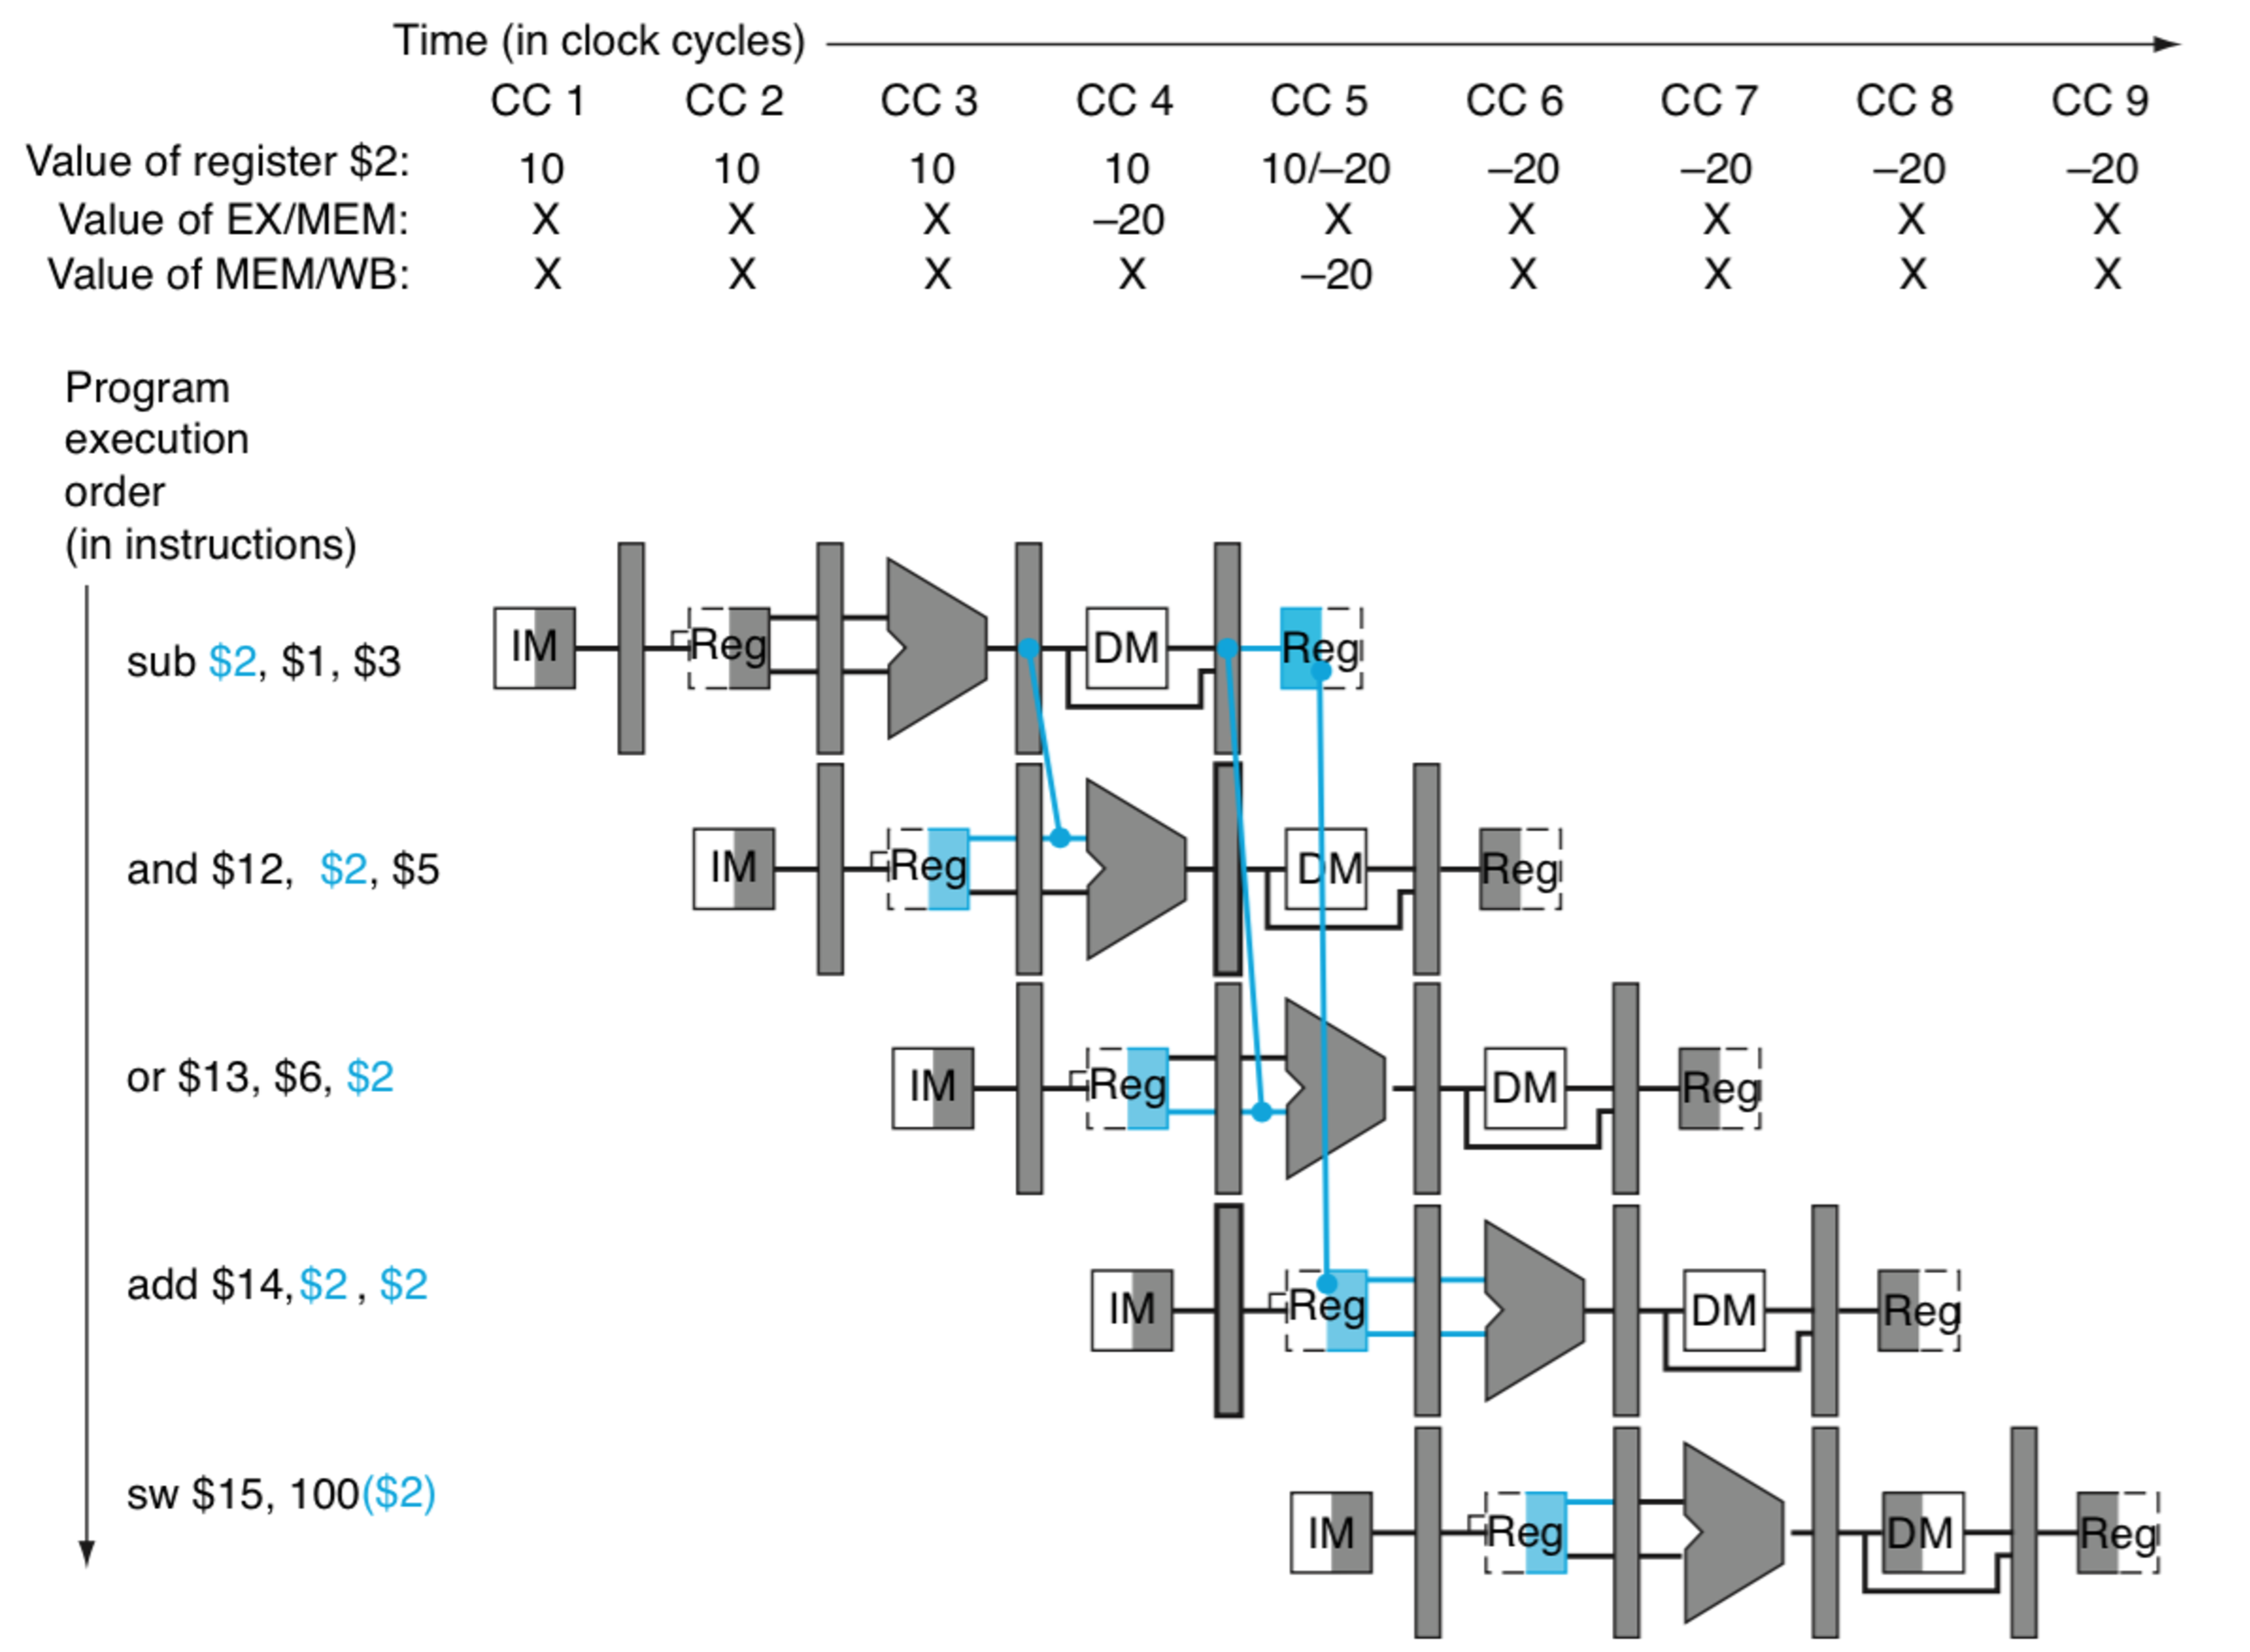
\includegraphics[width=6in]{./pics/pipelined-processor-forwarding}
\caption{An example of data dependencies that can be resolved by forwarding. This avoids data hazards \cite{Patterson2012}.}
\label{fig:pipelinedprocessorforwarding}
\end{figure}
%    dependencies resolution
%    Figure 6.29, Patterson2005, pp. 408
%    Figure 4.53, Patterson2012, pp. 367

%Figure \ref{fig:pipelinedprocessorrawdatadependencies} shows an example of Read-After-Write (RAW) data dependencies \cite{Hennessy2012,Shen2005a} between instructions in a snippet of a computer program \cite{Patterson2012}. There exist Read-After-Write (RAW) data dependencies \cite{Hennessy2012,Shen2005a} regarding register {\tt \$2} between the instruction {\tt sub \$2, \$1, \$3} and the following instructions: {\tt and \$12, \$2, \$5}; {\tt or \$13, \$6, \$2}; {\tt add \$14, \$2, \$2}; and {\tt sw \$15, 100(\$2)}. Figure \ref{fig:pipelinedprocessorforwarding} shows how these data dependencies can be resolved by forwarding dependent data from a datapath component to another datapath component in the same or next clock cycle. For example, there exists RAW data dependencies \cite{Hennessy2012,Shen2005a} regarding register {\tt \$2} between the instruction {\tt sub \$2, \$1, \$3} and the following instructions: {\tt and \$12, \$2, \$5}; {\tt or \$13, \$6, \$2}; and {\tt add \$14, \$2, \$2}. Therefore, forwarding is used to transfer the updated value of register {\tt \$2} to: the input of the ALU for the instruction {\tt and \$12, \$2, \$5}; the input of the ALU for the instruction {\tt or \$13, \$6, \$2}; and the register file at {\tt add \$14, \$2, \$2}. The RAW data dependency for register {\tt \$2} in last instruction {\tt sw \$15, 100(\$2)} will not cause a data hazard, since the value at register {\tt \$2} will be ready to be read from the register file at cycle six.
An extensive coverage of pipeline hazards is beyond the scope of this report. However, I will briefly address data dependencies and data hazards. Figure \ref{fig:pipelinedprocessorrawdatadependencies} shows an example of Read-After-Write (RAW) data dependencies \cite{Hennessy2012,Shen2005a} between instructions in a snippet of a computer program \cite{Patterson2012}. There exist Read-After-Write (RAW) data dependencies \cite{Hennessy2012,Shen2005a} regarding register {\tt \$2} between the instruction {\tt sub \$2, \$1, \$3} and the following instructions: {\tt and \$12, \$2, \$5}; {\tt or \$13, \$6, \$2}; {\tt add \$14, \$2, \$2}; and {\tt sw \$15, 100(\$2)}. Figure \ref{fig:pipelinedprocessorforwarding} shows how these data dependencies can be resolved by forwarding dependent data from a datapath component to another datapath component in the same or next clock cycle \cite{Patterson2012}. For example, there exists RAW data dependencies \cite{Hennessy2012,Shen2005a} regarding register {\tt \$2} between the instruction {\tt sub \$2, \$1, \$3} and the following instructions: {\tt and \$12, \$2, \$5}; {\tt or \$13, \$6, \$2}; and {\tt add \$14, \$2, \$2}. Therefore, forwarding is used to transfer the updated value of register {\tt \$2} to: the input of the ALU for the instruction {\tt and \$12, \$2, \$5}; the input of the ALU for the instruction {\tt or \$13, \$6, \$2}; and the register file at {\tt add \$14, \$2, \$2}. The RAW data dependency for register {\tt \$2} in last instruction {\tt sw \$15, 100(\$2)} will not cause a data hazard, since the value at register {\tt \$2} will be ready to be read from the register file at cycle six. \\


\begin{figure}[h]
\centering 
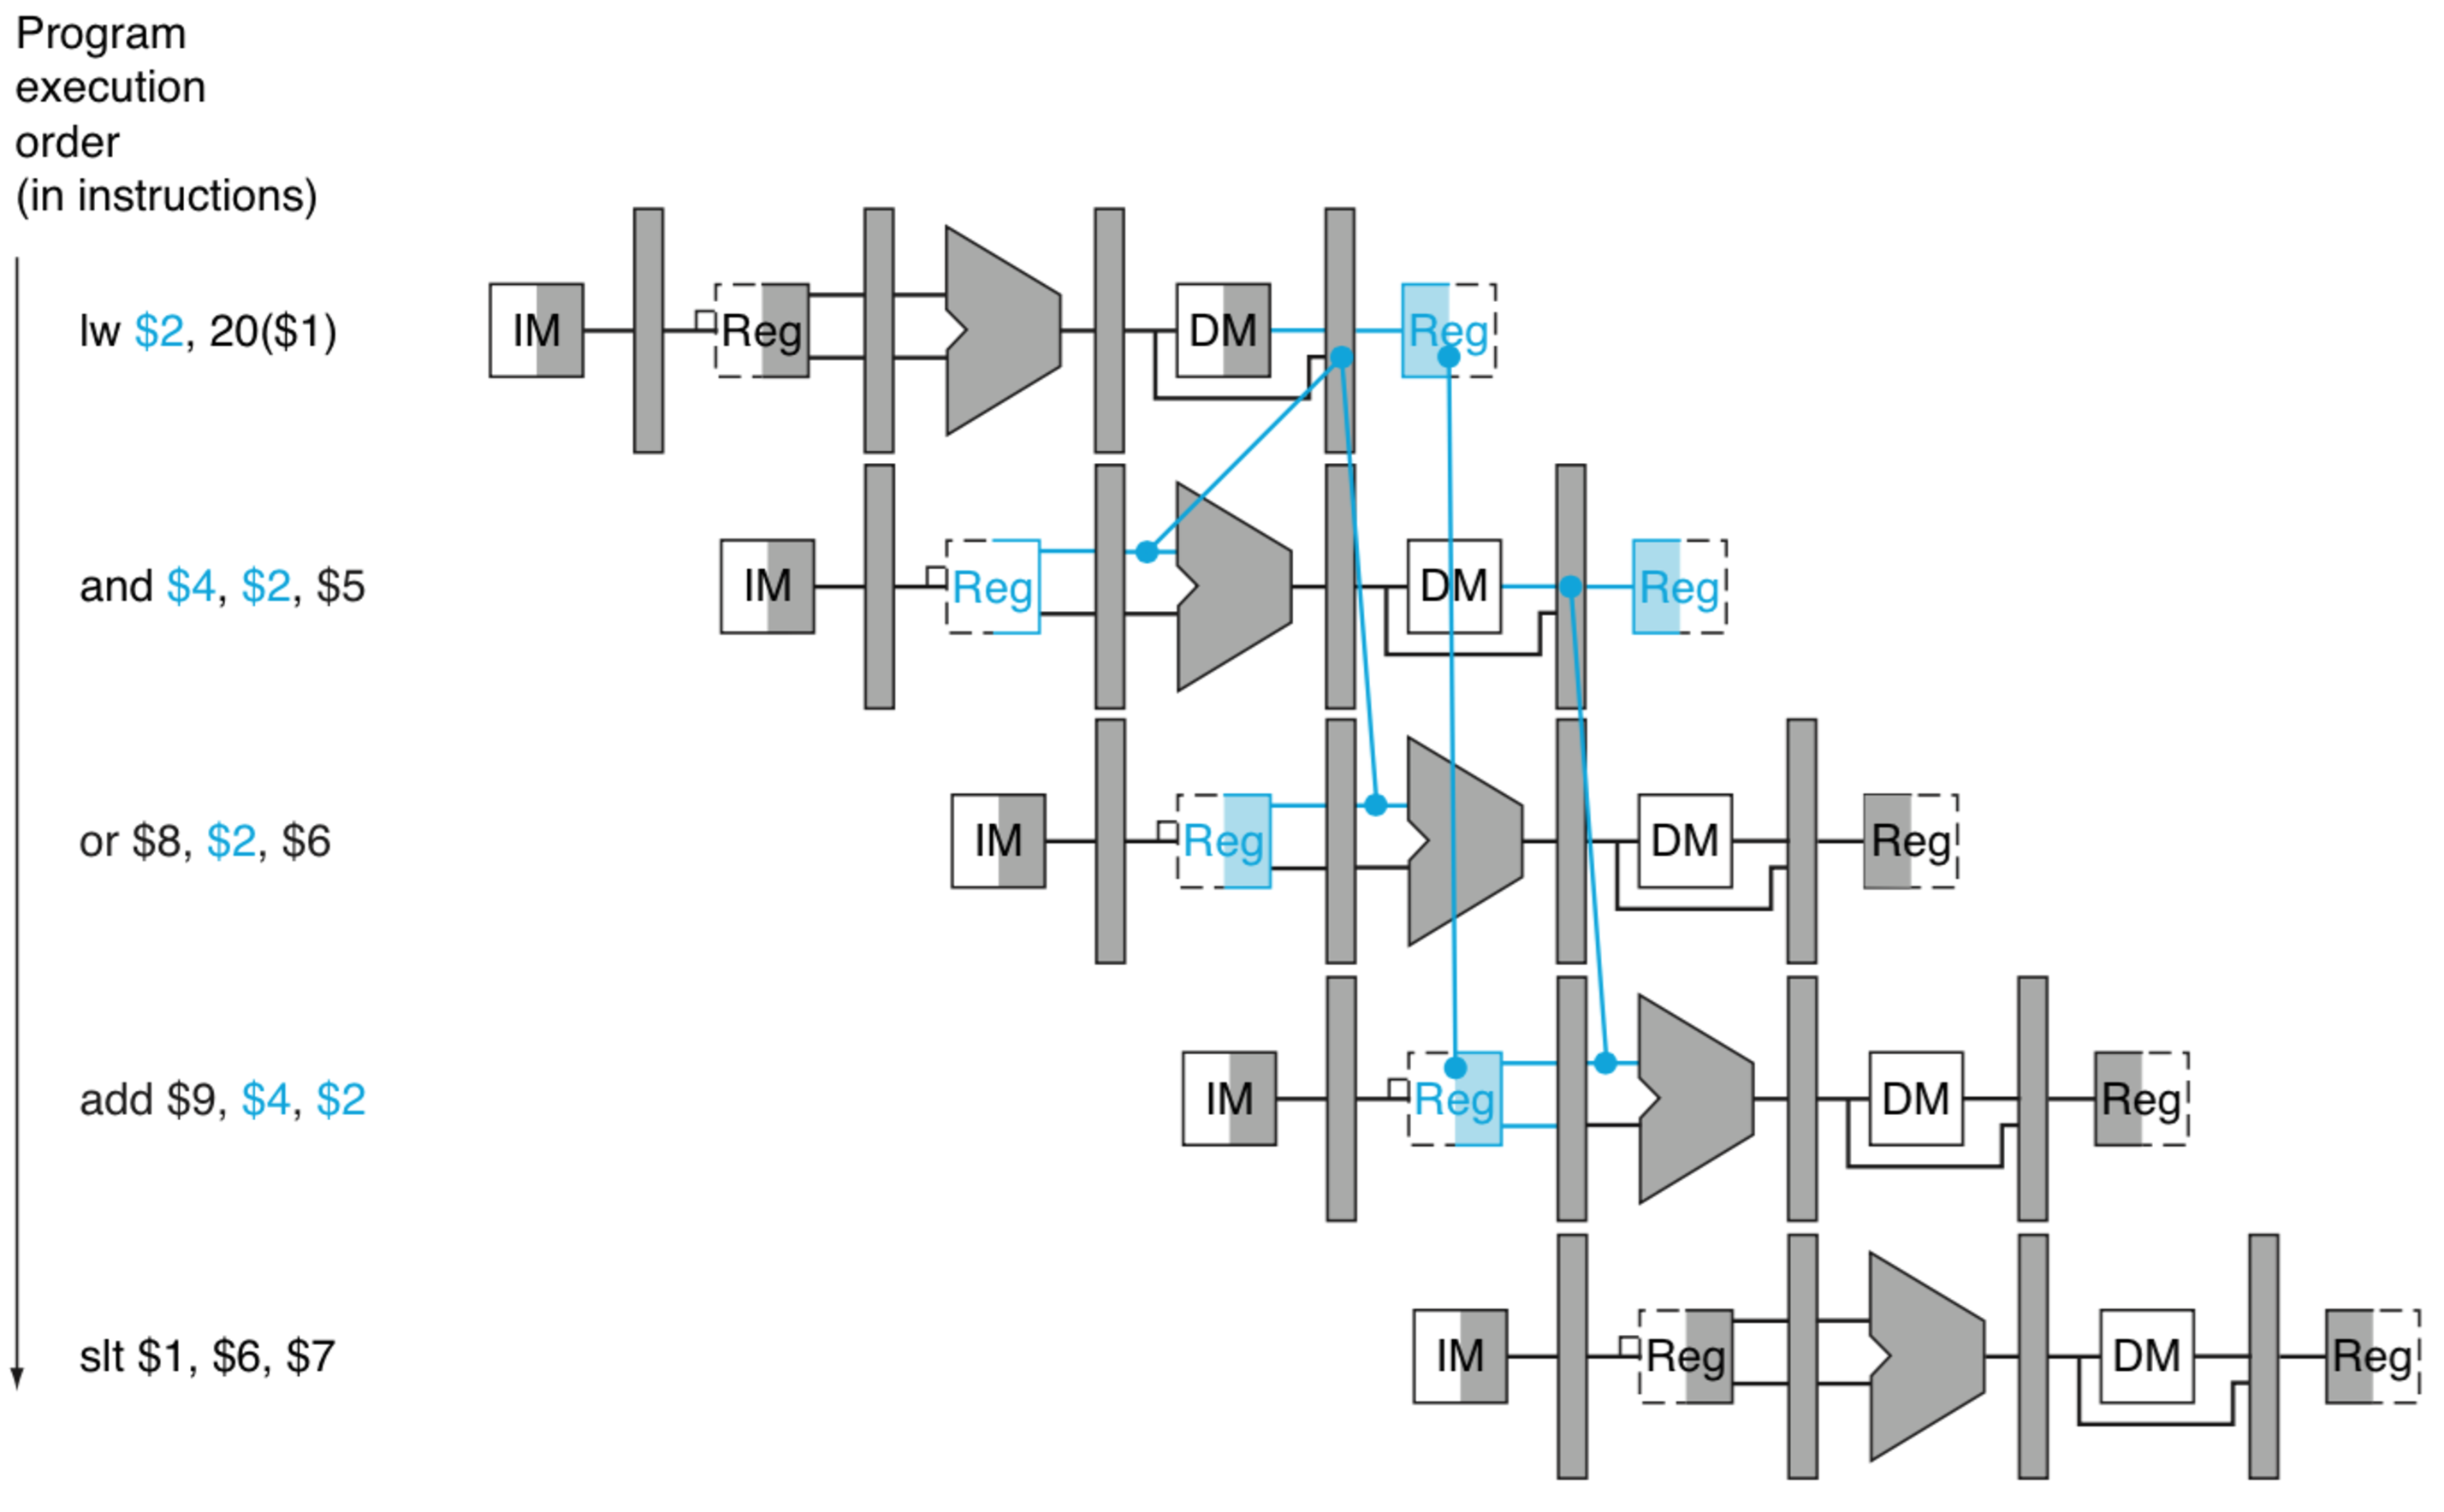
\includegraphics[width=6in]{./pics/pipelined-processor-data-hazards}
\caption{An example of data dependencies that cannot be resolved by forwarding and will cause data hazards \cite{Patterson2012}.}
\label{fig:pipelined-processor-data-hazards}
\end{figure}

\begin{figure}[h]
\centering 
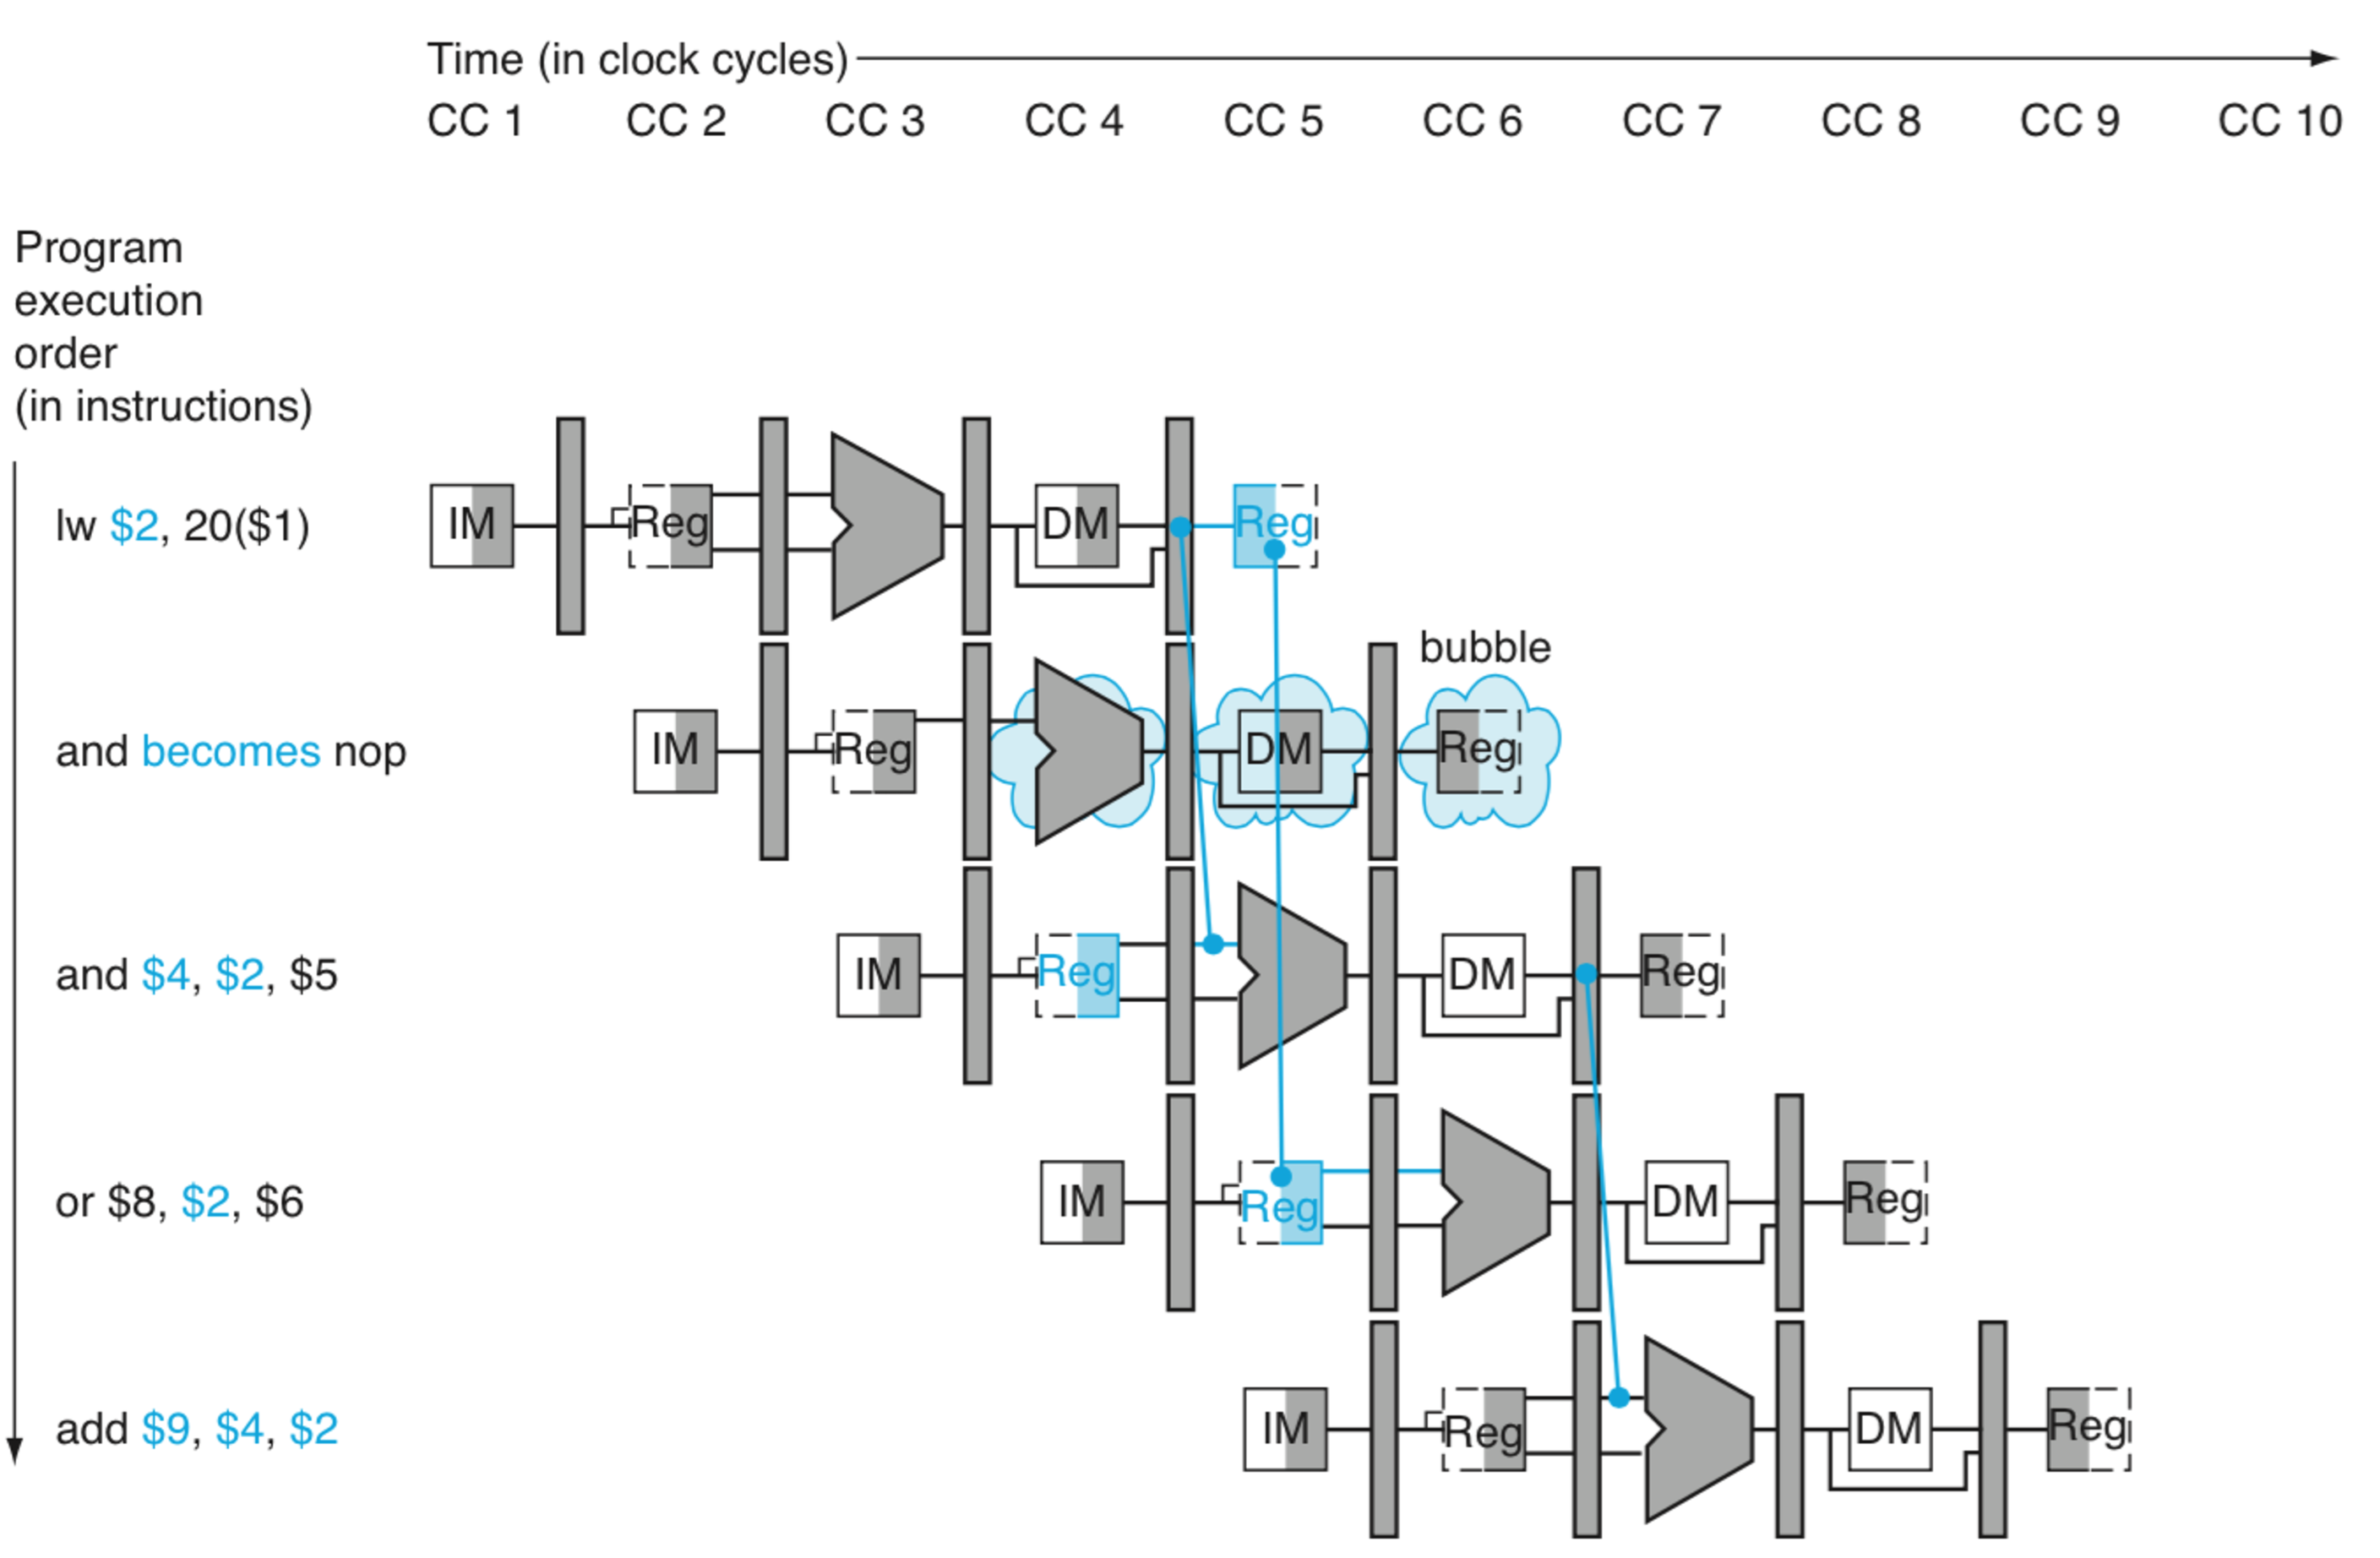
\includegraphics[width=6in]{./pics/pipelined-processor-bubbles}
\caption{An example of how bubbles/stalls can be inserted into a pipelined {\it MIPS} processor to avoid data hazards \cite{Patterson2012}.}
\label{fig:pipelinedprocessorbubbles}
\end{figure}
%    bubbles
%    Figure 6.34, Patterson2005, pp. 414
%    Figure 6.35, Patterson2005, pp. 415
%    Figure 4.58, Patterson2012, pp. 372
%    Figure 4.59, Patterson2012, pp. 374

Figure \ref{fig:pipelined-processor-data-hazards} shows an example of how some data dependencies cannot be resolved by forwarding of data values to another datapath component and these data dependencies will cause data hazards.
The register {\tt \$2} is written by the {\tt lw} instruction and is ready at the end of the fifth cycle. However, it is also required in the subsequent two instructions {\tt and} and {\tt or} in previous cycles. Hence, the data dependencies between these instructions have caused data hazards that will affect the correct functionality of the processor. To address the problem of data hazards, bubbles are used to delay the execution of instructions by flushing contents of the datapath pipeline that are associated with instructions causing these data hazards. Figure \ref{fig:pipelinedprocessorbubbles} shows how bubbles/stalls can be inserted into the datapath pipeline of a pipelined {\it MIPS} processor to avoid data hazards \cite{Patterson2012}. Bubbles (or {\tt nop} instructions) are inserted to flush contents of the ALU, memory device, and associated {\tt \$2} register in the register file. \\


Lastly, to improve the performance of pipelined processors regarding control hazards, techniques based on static branch prediction and dynamic branch prediction can be used. The former category of branch prediction techniques are carried out by compilers during compilation time, while the latter category of branch prediction techniques are carried out at run-time by the branch prediction unit in the pipelined microarchitecture \cite{Hennessy2012,Shen2005a}.






